% Provenance (never printed): see sources/outline_sources.md (Year 2: index minerals and zones,
% geothermometers and geobarometers, prograde and retrograde paths, metamorphic series,
% ultrahigh-pressure rocks and exhumation, ocean-floor metamorphism). Garnet-biotite
% calibration refitted from the Ferry and Spear (1978) brackets tabulated by Holdaway et al.
% (1997); GASP from Koziol and Newton (1988); thickening model after England and Thompson
% (1984) in figdata/bachelor-2/ptpaths.py; exercise and problem values in the Book 4 scratch
% calculators calc/ch11.py and calc/ch11b.py.
\chapter{Thermobarométrie et chemins P--T--t}\label{ch:b2:pt-paths}

Un grenat de quelques millimètres, cristallisé dans un schiste, conserve dans son cœur la composition
qu'il avait au début de sa croissance et dans sa bordure celle qu'il avait à son arrêt. Chaque
zone était en équilibre avec la biotite et le plagioclase qui l'entouraient, et la
façon dont le fer, le magnésium et le calcium se répartissaient entre ces minéraux dépend de la température
et de la pression. Lu à la lumière de la thermodynamique du chapitre précédent, un grenat dit
à quelle profondeur sa roche fut enfouie et jusqu'à quelle température elle s'est échauffée~; daté, il dit quand, et à quelle vitesse la
roche est remontée. Ce chapitre fait des minéraux métamorphiques des thermomètres, des baromètres
et des horloges, et suit une roche le long de son chemin à travers la croûte.

\begin{recall}
\textbf{Du volume de lycée}~: grade métamorphique, minéraux indicateurs et isogrades.
\textbf{Du volume de première année universitaire}~: le géotherme et la production de chaleur radiogénique~; la
croûte continentale d'environ \qty{35}{km} d'épaisseur~; datation radiométrique, la température de fermeture
d'un minéral et l'âge de refroidissement qu'il donne~; la croûte océanique et sa \omterm{def:b2:mantle-melting:peridotites}{péridotite}.
\textbf{Des volumes de physique}~: l'équation de la chaleur $\partial T/\partial t = \kappa\,
\partial^2 T/\partial z^2$ et la diffusivité thermique $\kappa$. \textbf{Des volumes de
chimie}~: la constante d'équilibre, $\Delta_r G^\circ + RT\ln K = 0$, et les activités dans
les solutions idéales. \textbf{Du \cref{ch:b2:metamorphic-facies}}~: \omterm{def:b2:metamorphic-facies:reaction}{réactions métamorphiques},
la \omterm{def:b2:metamorphic-facies:clapeyron}{pente de Clapeyron}, le diagramme de \ce{Al2SiO5} et les faciès.
\end{recall}
% ledger: prem:moho-average

\section{Zones métamorphiques}\label{sec:b2:pt-paths:zones}

Dans les argilites des Hautes-Terres d'Écosse, George Barrow cartographia dans les années 1890 une suite de
zones, chacune marquée par la première apparition d'un nouveau minéral indicateur. En allant vers
les grades plus élevés, la chlorite est rejointe tour à tour par la biotite, le grenat, la staurolite, la disthène et la sillimanite~;
dans les coupes types, les zones du grenat à la sillimanite se sont formées vers 500 à
\qty{650}{\celsius} et 5 à \qty{7}{kbar}.
% ledger: iugs:barrow, barrow1893:paper, earle:regional

\begin{definition}[Zones de Barrow~; gradient métamorphique de terrain]\label{def:b2:pt-paths:barrovian}
Les \emph{zones de Barrow}\index{zones de Barrow} sont les zones métamorphiques des
\omterm{def:b2:metamorphic-facies:protoliths}{métapélites} dans l'ordre chlorite, biotite, grenat, staurolite, disthène, sillimanite,
chacune commençant à l'isograde de son minéral indicateur. Le \emph{gradient métamorphique
de terrain}\index{gradient métamorphique de terrain} d'une région est la courbe, dans le
plan pression--température, passant par les conditions au pic enregistrées par ses roches aux
endroits où elles affleurent aujourd'hui.
\end{definition}

Chaque point d'un \omterm{def:b2:pt-paths:barrovian}{gradient métamorphique de terrain} vient d'une roche différente, et chaque roche a atteint son
pic à un moment qui lui est propre~: le gradient n'est pas le géotherme d'un instant donné, ni le
chemin d'une roche donnée. C'est la trace que laissent les pics sur la surface d'érosion actuelle.

\begin{omfigure}
\centering
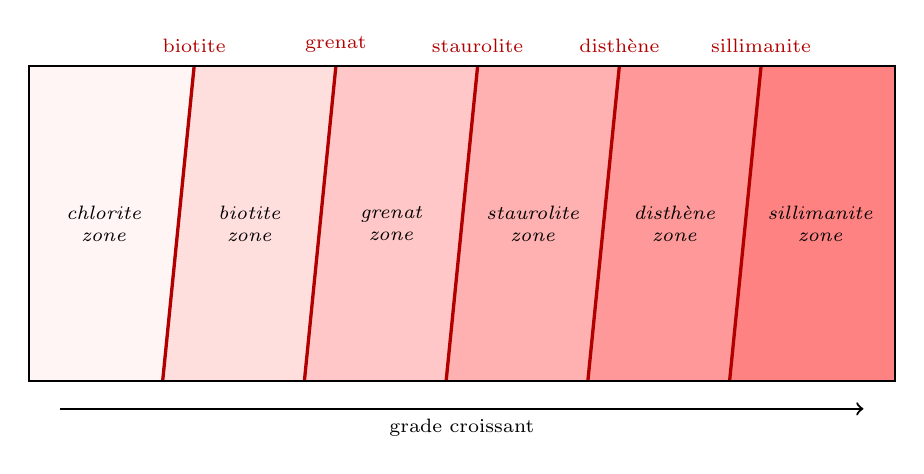
\begin{tikzpicture}[x=1cm, y=1cm]
\def\iso{{0,1.9,3.7,5.5,7.3,9.1,11}}
\foreach \i [evaluate=\i as \op using 4+9*\i] in {0,...,5} {
  \pgfmathsetmacro{\xa}{\iso[\i]}\pgfmathsetmacro{\xb}{\iso[\i+1]}
  \pgfmathsetmacro{\da}{(\i>0)*0.2}\pgfmathsetmacro{\db}{(\i<5)*0.2}
  \fill[red!\op!white] (\xa-\da,0) -- (\xb-\db,0) -- (\xb+\db,4) -- (\xa+\da,4) -- cycle;
}
\foreach \x/\n in {1.9/biotite, 3.7/grenat, 5.5/staurolite, 7.3/disthène, 9.1/sillimanite} {
  \draw[very thick, red!70!black] (\x-0.2,0) -- (\x+0.2,4);
  \node[font=\scriptsize, red!70!black, anchor=south] at (\x+0.2,4.05) {\n};
}
\draw[thick] (0,0) rectangle (11,4);
\foreach \x/\z in {0.95/chlorite, 2.8/biotite, 4.6/grenat, 6.4/staurolite, 8.2/disthène, 10.05/sillimanite}
  \node[font=\scriptsize\itshape, align=center] at (\x,2) {\z\\zone};
\draw[->, thick] (0.4,-0.35) -- node[below, font=\scriptsize] {grade croissant} (10.6,-0.35);
\end{tikzpicture}
\par\smallskip{\small \omterm{def:b2:pt-paths:barrovian}{Zones de Barrow} sur une carte, schématiques. Chaque isograde (trait rouge, nommé
au-dessus de la carte) est la ligne où son minéral indicateur apparaît pour la première fois~; le grade et la profondeur
de l'ombrage augmentent vers la droite. Chaque zone porte le nom du minéral qui apparaît à sa
limite de plus bas grade.}
\end{omfigure}
% ledger: iugs:barrow

Les isogrades sont cartographiés à partir des apparitions de minéraux, et ne deviennent des conditions de pression et
de température qu'une fois connues les réactions qui les sous-tendent. Pour aller plus loin, il faut
mesurer la température et la pression dans une seule roche.

\section{Thermomètres et baromètres}\label{sec:b2:pt-paths:thermobarometry}

\begin{definition}[Géothermomètre~; géobaromètre~; réaction d'échange~; réaction de transfert net]\label{def:b2:pt-paths:thermobarometry}
Un \emph{géothermomètre}\index{géothermomètre} (\emph{géobaromètre}\index{géobaromètre}) est
un équilibre entre minéraux dont la position dépend surtout de la température (de la pression), de sorte que
les compositions des minéraux donnent la température (la pression) de leur dernier
équilibre. Une \emph{réaction d'échange}\index{réaction d'échange} échange deux éléments
entre deux minéraux, comme le fer et le magnésium entre grenat et biotite, sans
créer ni détruire aucun des deux minéraux. Une \emph{réaction de transfert net}\index{réaction de transfert net}
forme certains minéraux aux dépens d'autres.
\end{definition}

Le thermomètre le plus utilisé pour les \omterm{def:b2:metamorphic-facies:protoliths}{métapélites} est l'échange de fer et de magnésium
entre grenat et biotite,
\[
\ce{Fe3Al2Si3O12 + KMg3AlSi3O10(OH)2 <=> Mg3Al2Si3O12 + KFe3AlSi3O10(OH)2},
\]
almandin plus phlogopite donnant pyrope plus annite. Soient $X_{\text{Mg}}$ et $X_{\text{Fe}}$
les fractions des sites occupés par le magnésium et le fer dans chaque minéral, et
\[
K_D = \frac{(X_{\text{Mg}}/X_{\text{Fe}})_{\text{grenat}}}{(X_{\text{Mg}}/X_{\text{Fe}})_{\text{biotite}}}.
\]
% ledger: h97:fs-reaction

\begin{proposition}[Un équilibre d'échange]\label{prop:b2:pt-paths:exchange}
Si le grenat et la biotite sont des solutions idéales et que $\Delta_r H$, $\Delta_r S$ et $\Delta_r V$ de
la réaction ci-dessus sont constants, alors à l'équilibre
\[
3RT\ln K_D = -(\Delta_r H + P\,\Delta_r V) + T\,\Delta_r S,
\qquad\text{donc}\qquad
T = \frac{\Delta_r H + P\,\Delta_r V}{\Delta_r S - 3R\ln K_D}.
\]
\end{proposition}

\begin{proof}
Chaque minéral possède trois sites pour le fer ou le magnésium. Dans une solution idéale, l'activité
d'un pôle est le produit des fractions de ses sites qu'il occupe~: $a_{\text{pyrope}} =
X_{\text{Mg}}^3$ dans le grenat, et ainsi de suite. La constante d'équilibre vaut donc
\[
K = \frac{a_{\text{pyrope}}\,a_{\text{annite}}}{a_{\text{almandine}}\,a_{\text{phlogopite}}}
= \frac{X_{\text{Mg,grt}}^3\,X_{\text{Fe,bt}}^3}{X_{\text{Fe,grt}}^3\,X_{\text{Mg,bt}}^3} = K_D^3 .
\]
À l'équilibre $\Delta_r G^\circ(T, P) + RT\ln K = 0$, avec $\Delta_r G^\circ = \Delta_r H -
T\,\Delta_r S + P\,\Delta_r V$ (le 1 de $P - 1$ étant négligé), ce qui donne la première équation~;
la résolution en $T$ donne la seconde.
\end{proof}

Les constantes proviennent d'expériences où du grenat et de la biotite synthétiques échangeaient du fer
et du magnésium à température connue et sous \qty{2.07}{kbar}. Douze encadrements de ce type, de 550 à
\qty{800}{\celsius}, portés en $\ln K_D$ en fonction de $1/T$, tombent près d'une droite (la figure
ci-dessous)~; par moindres carrés, avec $\Delta_r V = \qty{0.311}{J.bar^{-1}}$, on obtient
$\Delta_r H = \qty{52630}{J}$ et $\Delta_r S = \qty{20.19}{J.K^{-1}}$, les valeurs des
recalculs publiés des mêmes données. À plus haute température, le rapport $K_D$ monte
vers 1~: le grenat retient une plus grande part du magnésium.
% ledger: h97:fs-data, h97:ideal, h97:fs-reaction

\begin{omfigure}
\centering
\begin{tikzpicture}
\begin{axis}[omrecord, width=0.62\linewidth, height=5.2cm,
  xmin=0.9, xmax=1.25, ymin=-1.9, ymax=-1.1,
  xlabel={$1000/T$ (\unit{K^{-1}})}, ylabel={$\ln K_D$},
  tick label style={font=\scriptsize}, label style={font=\small},
  x tick label style={/pgf/number format/.cd, fixed, precision=2}]
\addplot[only marks, mark=*, mark size=1.6pt, blue!70!black]
  table[x expr={1000/(\thisrow{T_C}+273.15)}, y=lnKD] {figdata/out/bachelor-2-ptpaths-fs.dat};
\addplot[thick, red!75!black, domain=0.9:1.25, samples=2] {(-52630-2070*0.311)/(3*8.31441)*x/1000 + 20.19/(3*8.31441)};
\end{axis}
\end{tikzpicture}
\par\smallskip{\small Échange grenat--biotite~: les douze encadrements expérimentaux à
\qty{2.07}{kbar} (en bleu, tels que tabulés par Holdaway et ses coauteurs, 1997) et la droite de
la proposition, avec les $\Delta_r H$ et $\Delta_r S$ ajustés (en rouge).}
\end{omfigure}
% ledger: h97:fs-data, h97:ideal

Pour $K_D = 0.18$ à \qty{5}{kbar}, $T = (52630 + 0.311\times5000)/(20.19 - 3\times8.314
\times\ln 0.18) = 54185/62.96 = \qty{861}{K}$, soit \qty{587}{\celsius}. Un kilobar de plus
ajoute $0.311\times1000/62.96 = \qty{4.9}{K}$~: la réaction échange des ions de même charge
entre des sites de taille presque identique, sa variation de volume est faible, et la pression
joue à peine. C'est ce qui en fait un thermomètre.

Un baromètre demande l'inverse~: une réaction à forte variation de volume. La
\omterm{def:b2:pt-paths:thermobarometry}{réaction de transfert net}
\[
\ce{3 CaAl2Si2O8 <=> Ca3Al2Si3O12 + 2 Al2SiO5 + SiO2},
\]
l'anorthite donnant grossulaire, disthène et quartz, tasse les atomes de trois feldspaths en
minéraux plus denses~: $\Delta_r V = \qty{-6.21}{J.bar^{-1}}$, vingt fois celle de l'échange.
Son équilibre entre pôles, inversé dans des expériences entre 900 et \qty{1250}{\celsius} et 19
à \qty{28}{kbar}, suit la droite
\[
P_0 = 22.80\,T - 1093 \qquad (P_0 \text{ en bar}, T \text{ en } \unit{\celsius}).
\]
Dans une roche, le grossulaire est une petite part du grenat, et l'anorthite une part du
plagioclase. Avec des activités idéales, $a_{\text{grossulaire}} = X_{\text{Ca,grt}}^3$ et
$a_{\text{anorthite}} = X_{\text{an}}$, la condition $\Delta_r G^\circ + RT\ln K = 0$
écrite en $P$ et en $P_0$ donne
\[
P = P_0 + \frac{RT}{6.21}\,\ln\frac{X_{\text{Ca,grt}}^3}{X_{\text{an}}^3}
\qquad (T \text{ en kelvins dans le second terme}).
\]
Ce \omterm{def:b2:pt-paths:thermobarometry}{géobaromètre}, nommé GASP d'après les quatre minéraux (grenat, aluminosilicate, silice,
plagioclase), sert partout où une \omterm{def:b2:metamorphic-facies:protoliths}{métapélite} les renferme tous.
% ledger: kn88:gasp, rh95:gb-gasp

\begin{method}[Température et pression d'une roche]\label{met:b2:pt-paths:intersection}
(1) Mesurer, dans des minéraux qui ont cristallisé ensemble, les compositions que demandent le thermomètre et le
baromètre. (2) Supposer une pression et calculer la température avec le thermomètre.
(3) À cette température, calculer la pression avec le baromètre. (4) Recommencer (2) et (3)
jusqu'à ce que ni l'une ni l'autre ne change~; deux ou trois tours suffisent, car chaque équation dépend faiblement de
la variable que fixe l'autre. Graphiquement, la réponse est là où la droite du
thermomètre croise la droite du baromètre. (5) Propager les incertitudes~: pour
des erreurs indépendantes, $\sigma_T^2 = (\partial T/\partial\ln K_D)^2\sigma_{\ln K_D}^2 +
(\partial T/\partial P)^2\sigma_P^2$, et de même pour $P$.
\end{method}

\begin{omfigure}
\centering
\begin{tikzpicture}
\begin{axis}[omrecord, width=0.78\linewidth, height=6.4cm,
  xmin=400, xmax=800, ymin=0, ymax=12, xlabel={$T$ (\unit{\celsius})}, ylabel={$P$ (\unit{kbar})},
  tick label style={font=\scriptsize}, label style={font=\small}, clip=false]
\addplot[thick, red!75!black] table[x=kd12, y=P_kbar] {figdata/out/bachelor-2-ptpaths-gb.dat};
\addplot[thick, red!75!black] table[x=kd15, y=P_kbar] {figdata/out/bachelor-2-ptpaths-gb.dat};
\addplot[thick, red!75!black] table[x=kd18, y=P_kbar] {figdata/out/bachelor-2-ptpaths-gb.dat};
\addplot[thick, red!75!black] table[x=kd21, y=P_kbar] {figdata/out/bachelor-2-ptpaths-gb.dat};
\addplot[thick, red!75!black] table[x=kd24, y=P_kbar] {figdata/out/bachelor-2-ptpaths-gb.dat};
\addplot[thick, blue!70!black] table[x=T_C, y=r15] {figdata/out/bachelor-2-ptpaths-gasp.dat};
\addplot[thick, blue!70!black] table[x=T_C, y=r20] {figdata/out/bachelor-2-ptpaths-gasp.dat};
\addplot[thick, blue!70!black] table[x=T_C, y=r25] {figdata/out/bachelor-2-ptpaths-gasp.dat};
\addplot[thick, blue!70!black] table[x=T_C, y=r30] {figdata/out/bachelor-2-ptpaths-gasp.dat};
\node[font=\tiny, red!75!black, anchor=west] at (axis cs:452,0.5) {0.12};
\node[font=\tiny, red!75!black, anchor=west] at (axis cs:511,0.5) {0.15};
\node[font=\tiny, red!75!black, anchor=west] at (axis cs:568,0.5) {0.18};
\node[font=\tiny, red!75!black, anchor=west] at (axis cs:622,0.5) {0.21};
\node[font=\tiny, red!75!black, anchor=west] at (axis cs:675,0.5) {0.24};
\node[font=\tiny, blue!70!black, anchor=west] at (axis cs:802,8.97) {0.15};
\node[font=\tiny, blue!70!black, anchor=west] at (axis cs:802,10.21) {0.20};
\node[font=\tiny, blue!70!black, anchor=west] at (axis cs:802,11.17) {0.25};
\node[font=\tiny, blue!70!black, anchor=west] at (axis cs:802,11.96) {0.30};
\end{axis}
\end{tikzpicture}
\par\smallskip{\small Isothermes grenat--biotite (rouges, raides, étiquetées par $K_D$) et isobares GASP
(bleues, étiquetées à droite par le rapport $X_{\text{Ca}}/X_{\text{an}}$ du
grossulaire dans le grenat à l'anorthite dans le plagioclase), issues des calibrations de cette section. Une roche qui renferme les deux couples se place
là où ses deux droites se croisent.}
\end{omfigure}
% ledger: h97:ideal, h97:fs-reaction, kn88:gasp

Les droites du thermomètre sont presque verticales, celles du baromètre inclinées~: elles se croisent sous un
grand angle, ce qui rend l'intersection précise. Le mélange idéal est la simplification principale
de ce chapitre. Les vrais grenats renferment du calcium et du manganèse, les vraies biotites de l'aluminium,
du titane et du fer ferrique, et les calibrations qui en tiennent compte décalent les températures de
plusieurs dizaines de degrés (dans une région bien étudiée, \qty{574}{\celsius} au lieu de
\qty{530}{\celsius})~; les meilleures revendiquent une incertitude d'environ \qty{25}{\celsius}.
% ledger: h97:ideal, h97:corrections

\section{Chemins pression--température}\label{sec:b2:pt-paths:paths}

Une roche n'atteint pas sa pression maximale et sa température maximale au même instant.
Elle est enfouie et réchauffée, puis ramenée vers la surface et refroidie, et ses minéraux réagissent tout
au long du trajet.

\begin{definition}[Chemin P--T~; chemins prograde et rétrograde~; conditions au pic du métamorphisme]\label{def:b2:pt-paths:paths}
Le \emph{chemin P--T}\index{chemin P--T} d'une roche est la suite des pressions et
des températures qu'elle a traversées au cours d'un événement métamorphique. Son \emph{chemin
prograde}\index{chemin prograde} est la portion le long de laquelle la température monte, son \emph{chemin
rétrograde}\index{chemin rétrograde}, la portion où elle descend. Les \emph{conditions
au pic du métamorphisme}\index{conditions au pic du métamorphisme} sont la pression et la température à la
plus haute température du chemin, le pic thermique~; le pic de pression, ou pic barique, ne
coïncide pas forcément avec lui.
\end{definition}
% ledger: scmr:ptt

Un chemin est dit \emph{horaire} lorsque, tracé avec la température vers la droite et la pression vers le haut,
le pic thermique vient après le pic barique, pendant la décompression~; il est
\emph{antihoraire} lorsque le pic thermique est atteint alors que la pression augmente encore. Quel
sens suit une roche dépend de la manière dont la chaleur l'a atteinte, et le cas le plus simple peut être
calculé.
% ledger: scmr:ptt

Imaginons une croûte de \qty{35}{km} d'épaisseur, en régime permanent, avec une production de chaleur de
\qty{1.0}{\micro W.m^{-3}}, un flux de chaleur de \qty{25}{mW.m^{-2}} venant du dessous, une conductivité
de \qty{2.5}{W.m^{-1}.K^{-1}} et une diffusivité de \qty{1e-6}{m^2.s^{-1}}, ces trois valeurs
étant comprises dans les intervalles mesurés sur des roches. Son flux de chaleur en surface vaut \qty{60}{mW.m^{-2}} et son Moho se trouve à
\qty{595}{\celsius}. Une collision empile une seconde copie de cette croûte par-dessus, rapidement
au regard du temps que met la chaleur à se déplacer~: les roches de la nappe inférieure gardent leurs
températures mais se trouvent \qty{35}{km} plus bas, si bien que le géotherme devient une dent de scie, avec
des roches à \qty{0}{\celsius} à \qty{35}{km} sous des roches chaudes de la nappe supérieure. La croûte est
désormais épaisse de \qty{70}{km} et contient deux fois plus de roche productrice de chaleur. Trente millions d'années après
l'empilement, l'érosion commence et enlève \qty{35}{km} en 70 millions d'années
(\qty{0.5}{mm.an^{-1}}).
% ledger: delaney:conductivity, roy:granitic-k, vila:heat-production, prem:moho-average, et84:ptt

\begin{proposition}[Échelle de temps de la relaxation thermique]\label{prop:b2:pt-paths:relaxation}
Dans une couche d'épaisseur $L$ dont les deux faces sont maintenues à température fixe, une perturbation de température
de la forme $\sin(\pi z/L)$ décroît comme $e^{-t/\tau}$, avec
\[
\tau = \frac{L^2}{\pi^2\kappa}.
\]
\end{proposition}

\begin{proof}
Écrivons $\theta(z, t) = f(t)\sin(\pi z/L)$, qui s'annule en $z = 0$ et $z = L$. L'équation de la
chaleur $\partial\theta/\partial t = \kappa\,\partial^2\theta/\partial z^2$ donne
$f'\sin(\pi z/L) = -\kappa(\pi/L)^2 f\sin(\pi z/L)$, donc $f' = -f/\tau$ avec $\tau =
L^2/(\pi^2\kappa)$, et $f = f(0)\,e^{-t/\tau}$.
\end{proof}

La dent de scie a une longueur d'onde de l'ordre de l'épaisseur d'une nappe~: avec $L =
\qty{35}{km}$, $\tau = \qty{3.9}{Ma}$, et le coin froid à \qty{35}{km} est effacé en
dix millions d'années. La croûte épaissie entière, $L = \qty{70}{km}$, se relâche avec $\tau =
\qty{16}{Ma}$, de sorte que le réchauffement se poursuit pendant des dizaines de millions d'années, vers
le géotherme bien plus chaud que supporte une croûte deux fois plus épaisse, avec deux fois plus de roche
productrice de chaleur. La
figure ci-dessous montre les géothermes calculés.
% ledger: delaney:conductivity

\begin{omfigure}
\centering
\begin{tikzpicture}
\begin{axis}[omrecord, width=0.62\linewidth, height=6.6cm,
  xmin=0, xmax=1000, ymin=0, ymax=80, y dir=reverse,
  xlabel={$T$ (\unit{\celsius})}, ylabel={profondeur (\unit{km})},
  legend style={font=\scriptsize, at={(0.02,0.02)}, anchor=south west},
  tick label style={font=\scriptsize}, label style={font=\small}]
\addplot[thick, black] table[x=t0, y=z_km] {figdata/out/bachelor-2-ptpaths-geo.dat};
\addlegendentry{\qty{0}{Ma}}
\addplot[thick, blue!70!black] table[x=t10, y=z_km] {figdata/out/bachelor-2-ptpaths-geo.dat};
\addlegendentry{\qty{10}{Ma}}
\addplot[thick, orange!85!black] table[x=t30, y=z_km] {figdata/out/bachelor-2-ptpaths-geo.dat};
\addlegendentry{\qty{30}{Ma}}
\addplot[thick, red!75!black] table[x=t60, y=z_km] {figdata/out/bachelor-2-ptpaths-geo.dat};
\addlegendentry{\qty{60}{Ma}}
\end{axis}
\end{tikzpicture}
\par\smallskip{\small Géothermes après doublement d'une croûte de \qty{35}{km} par empilement, calculés
avec l'équation de la chaleur (profondeurs sous la surface à l'instant considéré~; l'érosion commence à
\qty{30}{Ma}). En noir~: la dent de scie juste après l'empilement. La base de la croûte épaissie,
à \qty{595}{\celsius} au départ, dépasse \qty{900}{\celsius} au bout de 60 millions d'années.}
\end{omfigure}
% ledger: et84:ptt

Suivons la roche qui se trouvait en surface avant l'empilement et qui se trouve à \qty{35}{km} juste
après, sous \qty{9.6}{kbar}. En cinq millions d'années, elle se réchauffe de 0 à
\qty{395}{\celsius} sans bouger~; au début de l'érosion, elle a atteint
\qty{558}{\celsius}. L'érosion la remonte ensuite, mais la chaleur arrive encore plus vite
que la roche ne s'échappe~: elle se réchauffe encore lorsqu'elle est remontée de \qty{6}{km}, et atteint son
pic thermique, \qty{593}{\celsius} à \qty{7.8}{kbar}, 43 millions d'années après l'empilement. Ce n'est
qu'alors qu'elle se refroidit, en passant par \qty{405}{\celsius} à \qty{13}{km} de profondeur, et
\qty{74}{Ma}, en route vers la surface. Le chemin (figure ci-dessous) est horaire. Il reste aussi
à moins de \qty{50}{\celsius} de sa température de pic pendant trente millions d'années, soit environ un
tiers de son trajet complet, comme l'ont trouvé England et Thompson en 1984 pour la plupart des cas
géologiquement plausibles~: une roche passe longtemps près de son pic, et les minéraux qu'elle conserve
enregistrent surtout cette étape.
% ledger: et84:ptt

\begin{omfigure}
\centering
\begin{tikzpicture}
\begin{axis}[omrecord, width=0.78\linewidth, height=6.2cm,
  xmin=0, xmax=800, ymin=0, ymax=11, xlabel={$T$ (\unit{\celsius})}, ylabel={$P$ (\unit{kbar})},
  tick label style={font=\scriptsize}, label style={font=\small}]
\addplot[thick, gray, densely dashed, restrict x to domain=0:504] table[x=T_C, y=P_kbar] {figdata/out/bachelor-2-facies-hm93-kyand.dat};
\addplot[thick, gray, densely dashed] table[x=T_C, y=P_kbar] {figdata/out/bachelor-2-facies-hm93-kysil.dat};
\addplot[thick, gray, densely dashed] table[x=T_C, y=P_kbar] {figdata/out/bachelor-2-facies-hm93-andsil.dat};
\addplot[very thick, red!75!black, postaction={decorate}, decoration={markings,
  mark=at position 0.2 with {\arrow{Stealth[length=2.5mm]}},
  mark=at position 0.52 with {\arrow{Stealth[length=2.5mm]}},
  mark=at position 0.8 with {\arrow{Stealth[length=2.5mm]}}}] table[x=T_C, y=P_kbar] {figdata/out/bachelor-2-ptpaths-path.dat};
\node[font=\scriptsize\bfseries, gray] at (axis cs:330,6.5) {disthène};
\node[font=\scriptsize\bfseries, gray] at (axis cs:520,1.0) {andalousite};
\node[font=\scriptsize\bfseries, gray] at (axis cs:740,4.0) {sillimanite};
\node[font=\scriptsize, red!75!black, anchor=south] at (axis cs:200,9.7) {chauffage en profondeur};
\node[font=\scriptsize, red!75!black, anchor=west] at (axis cs:603,8.9) {pic thermique};
\node[font=\scriptsize, red!75!black, anchor=west] at (axis cs:110,2.7) {remontée avec refroidissement};
\end{axis}
\end{tikzpicture}
\par\smallskip{\small \omterm{def:b2:pt-paths:paths}{Chemin P--T} de la roche qui se trouve à \qty{35}{km} juste après la
empilement (en rouge, échantillonné tous les deux millions d'années), calculé avec le modèle des géothermes ci-dessus,
sur le diagramme expérimental \ce{Al2SiO5} du \cref{ch:b2:metamorphic-facies} (en gris). Le
pic de pression vient en premier, le pic thermique pendant la décompression~: un chemin horaire, qui
ne quitte jamais le champ de la disthène.}
\end{omfigure}
% ledger: et84:ptt, hm93:table11

Le modèle montre aussi pourquoi certains chemins tournent dans l'autre sens. L'épaississement seul réchauffe une roche
seulement après qu'elle a été enfouie, si bien que son pic thermique survient pendant l'\omterm{def:b2:pt-paths:exhumation}{exhumation}. Une roche dont
la température monte alors qu'elle est encore enfouie a besoin de chaleur venue d'ailleurs, par exemple d'un \omterm{def:b2:magma-emplacement:magma}{magma}
remontant dans la croûte au-dessus ou à côté d'elle, et suit un chemin antihoraire. Et dans la
croûte épaissie, la base se réchauffe bien au-dessus de sa température initiale~: England et Thompson
concluent qu'une fusion importante de la croûte est une conséquence probable de l'épaississement,
qui fait l'objet du \cref{ch:b2:crustal-melting}.
% ledger: et84:ptt, scmr:ptt

\section{Ajouter le temps}\label{sec:b2:pt-paths:time}

\begin{definition}[Chemin P--T--t]\label{def:b2:pt-paths:ptt}
Le \emph{chemin P--T--t}\index{chemin P--T--t} d'une roche est son \omterm{def:b2:pt-paths:paths}{chemin P--T} auquel on associe l'instant
auquel chaque point a été atteint.
\end{definition}
% ledger: scmr:ptt

Le temps vient de la datation radiométrique. Un minéral qui a cristallisé pendant l'événement et conservé
ses isotopes fils depuis, comme une zone de grenat datée par la
méthode samarium--néodyme, date sa propre croissance, et sa
composition donne la pression et la température de ce moment. Un minéral qui a cristallisé
plus tôt, à plus haute température, donne au contraire un âge de refroidissement~: le moment où la roche
s'est refroidie à travers la température de fermeture de ce minéral et de ce système isotopique (volume de première année
universitaire). Pour l'argon dans un grain de muscovite de rayon \qty{100}{\micro m}, refroidi à
\qty{10}{\celsius} par million d'années, la température de fermeture vaut \qty{405}{\celsius} à
\qty{5}{kbar} et \qty{425}{\celsius} à \qty{10}{kbar}.
% ledger: h09:muscovite

\begin{definition}[Exhumation~; vitesse d'exhumation]\label{def:b2:pt-paths:exhumation}
\emph{Exhumation}\index{exhumation} est le mouvement d'une roche vers la surface de la Terre,
par enlèvement des roches qui la surmontent. La \emph{vitesse d'exhumation}\index{vitesse d'exhumation} est la
vitesse de diminution de sa profondeur.
\end{definition}

\begin{proposition}[Vitesses à partir de deux points datés]\label{prop:b2:pt-paths:rates}
Si une roche se trouvait à la température $T_1$ et à la profondeur $z_1$ à l'instant $t_1$, puis à $T_2$, $z_2$ à un
instant ultérieur $t_2$ (âges comptés à rebours depuis aujourd'hui, $t_1 > t_2$), ses vitesses moyennes de refroidissement et
d'\omterm{def:b2:pt-paths:exhumation}{exhumation} sur l'intervalle sont
\[
\frac{T_1 - T_2}{t_1 - t_2}
\qquad\text{et}\qquad
\frac{z_1 - z_2}{t_1 - t_2},
\]
Leurs incertitudes, pour des erreurs indépendantes sur les deux âges, découlent de
$\sigma_{t_1 - t_2}^2 = \sigma_{t_1}^2 + \sigma_{t_2}^2$.
\end{proposition}

\begin{proof}
Une vitesse moyenne est une différence divisée par le temps écoulé $t_1 - t_2$~; la variance d'une
différence de grandeurs indépendantes est la somme de leurs variances.
\end{proof}

La profondeur à laquelle un âge de refroidissement a été fixé est rarement mesurée~: on l'estime à partir du
géotherme de l'époque, ce qui explique que les \omterm{def:b2:pt-paths:exhumation}{vitesses d'exhumation} soient moins sûres que les vitesses de refroidissement.
Une pression, lorsqu'un \omterm{def:b2:metamorphic-facies:assemblage}{assemblage minéralogique} en donne une, fixe directement la profondeur, par
$z = P/(\bar\rho g)$, avec $\bar\rho$ la masse volumique moyenne des roches au-dessus.

\section{Séries métamorphiques et ceintures couplées}\label{sec:b2:pt-paths:series}

\begin{definition}[Série métamorphique~; ceintures métamorphiques couplées]\label{def:b2:pt-paths:series}
Une \emph{série métamorphique}\index{série métamorphique} (ou série de faciès) est une suite de
\omterm{def:b2:metamorphic-facies:facies}{faciès métamorphiques} développés dans la même gamme de rapports pression sur température,
occupant donc un secteur radial du plan pression--température.
Les \emph{ceintures métamorphiques couplées}\index{ceintures métamorphiques couplées} sont deux ceintures parallèles de
même âge, l'une de séries haute pression et l'autre de séries basse pression.
\end{definition}
% ledger: scmr:ptt, wallis24:paired

On distingue couramment trois séries. Un rapport pression sur température élevé, le long d'un
gradient froid, mène du faciès des zéolites aux schistes bleus et aux éclogites~: la série
des zones de subduction. Un rapport intermédiaire traverse les faciès schiste vert, amphibolite et
granulite, avec disthène puis sillimanite dans les \omterm{def:b2:metamorphic-facies:protoliths}{métapélites}~: la série de Barrow. Un rapport faible
le long de gradients chauds comme ceux qui bordent les intrusions, produit d'abord de l'andalousite puis
de la sillimanite~: la série basse pression, ou série de Buchan. La figure ci-dessous trace trois gradients
sur le diagramme des aluminosilicates.
% ledger: scmr:ptt, scmr:facies, iugs:barrow, fub:paired

\begin{omfigure}
\centering
\begin{tikzpicture}
\begin{axis}[omrecord, width=0.78\linewidth, height=6.2cm,
  xmin=0, xmax=900, ymin=0, ymax=12, xlabel={$T$ (\unit{\celsius})}, ylabel={$P$ (\unit{kbar})},
  tick label style={font=\scriptsize}, label style={font=\small}]
\addplot[thick, gray, densely dashed, restrict x to domain=0:504] table[x=T_C, y=P_kbar] {figdata/out/bachelor-2-facies-hm93-kyand.dat};
\addplot[thick, gray, densely dashed] table[x=T_C, y=P_kbar] {figdata/out/bachelor-2-facies-hm93-kysil.dat};
\addplot[thick, gray, densely dashed] table[x=T_C, y=P_kbar] {figdata/out/bachelor-2-facies-hm93-andsil.dat};
\addplot[very thick, blue!70!black] table[x=T_C, y=g10] {figdata/out/bachelor-2-ptpaths-series.dat};
\addplot[very thick, green!45!black] table[x=T_C, y=g25] {figdata/out/bachelor-2-ptpaths-series.dat};
\addplot[very thick, orange!85!black] table[x=T_C, y=g60] {figdata/out/bachelor-2-ptpaths-series.dat};
\node[font=\scriptsize, blue!70!black, rotate=52, anchor=south] at (axis cs:330,8.5) {\qty{10}{\celsius\per\km}};
\node[font=\scriptsize, green!45!black, rotate=28, anchor=south] at (axis cs:640,7.0) {\qty{25}{\celsius\per\km}};
\node[font=\scriptsize, orange!85!black, rotate=12, anchor=south] at (axis cs:800,3.65) {\qty{60}{\celsius\per\km}};
\node[font=\scriptsize\bfseries, gray] at (axis cs:120,5.5) {disthène};
\node[font=\scriptsize\bfseries, gray] at (axis cs:470,1.1) {andalousite};
\node[font=\scriptsize\bfseries, gray] at (axis cs:800,1.6) {sillimanite};
\end{axis}
\end{tikzpicture}
\par\smallskip{\small Trois gradients géothermiques depuis une surface à \qty{10}{\celsius},
convertis en pression avec une masse volumique moyenne de \qty{2800}{kg.m^{-3}}, sur le diagramme expérimental
\ce{Al2SiO5} (en gris). Le gradient froid reste dans le champ de la disthène, le
gradient intermédiaire passe de la disthène à la sillimanite, le gradient chaud traverse le champ de l'andalousite
avant d'atteindre la sillimanite.}
\end{omfigure}
% ledger: hm93:table11

L'idée des séries est venue du Japon, où Akiho Miyashiro les définit en 1961. Dans
le sud-ouest du pays, la ceinture de Sanbagawa, de \omterm{def:b2:metamorphic-facies:metamorphism}{métamorphisme} haute pression et basse température,
s'étend sur plus de \qty{800}{km} à côté de la ceinture de Ryoke, de \omterm{def:b2:metamorphic-facies:metamorphism}{métamorphisme} haute température et basse pression,
les deux étant séparées par une grande faille~: la paire classique. La
ceinture de Sanbagawa est une ancienne zone de subduction~; la ceinture de Ryoke en est l'arc volcanique. Une
zone de subduction produit ainsi les deux séries à la fois, des roches froides entraînées vers le bas par la plaque
qui plonge, des roches chauffées dans l'arc~; des ceintures couplées du même genre sont connues autour du
Pacifique.
% ledger: wallis24:paired, koguchi17:paired, fub:paired, scmr:ptt

\section{Ultra-haute pression et exhumation}\label{sec:b2:pt-paths:uhp}

En 1984 fut décrit un quartzite du massif de Dora Maira, dans les Alpes occidentales, dont les grenats,
jusqu'à \qty{25}{cm} de diamètre et presque purs en pyrope, renferment des grains de
coésite, la forme dense de la silice, partiellement retransformée en quartz~; la dilatation lors de
cette inversion a fracturé radialement le grenat hôte autour de chaque grain. La coésite et
ses compagnons impliquent au moins \qty{28}{kbar} vers \qty{700}{\celsius}~: des roches de la croûte
continentale supérieure, autrefois des sédiments, étaient descendues à \qty{90}{km} ou plus, puis
sont remontées.
% ledger: chopin84:coesite

\begin{definition}[Métamorphisme d'ultra-haute pression]\label{def:b2:pt-paths:uhp}
Le \emph{métamorphisme d'ultra-haute pression}\index{métamorphisme d'ultra-haute pression} est
le \omterm{def:b2:metamorphic-facies:metamorphism}{métamorphisme} de roches crustales à des pressions assez élevées pour que la coésite ou le diamant puissent croître.
\end{definition}

\begin{omfigure}
\centering
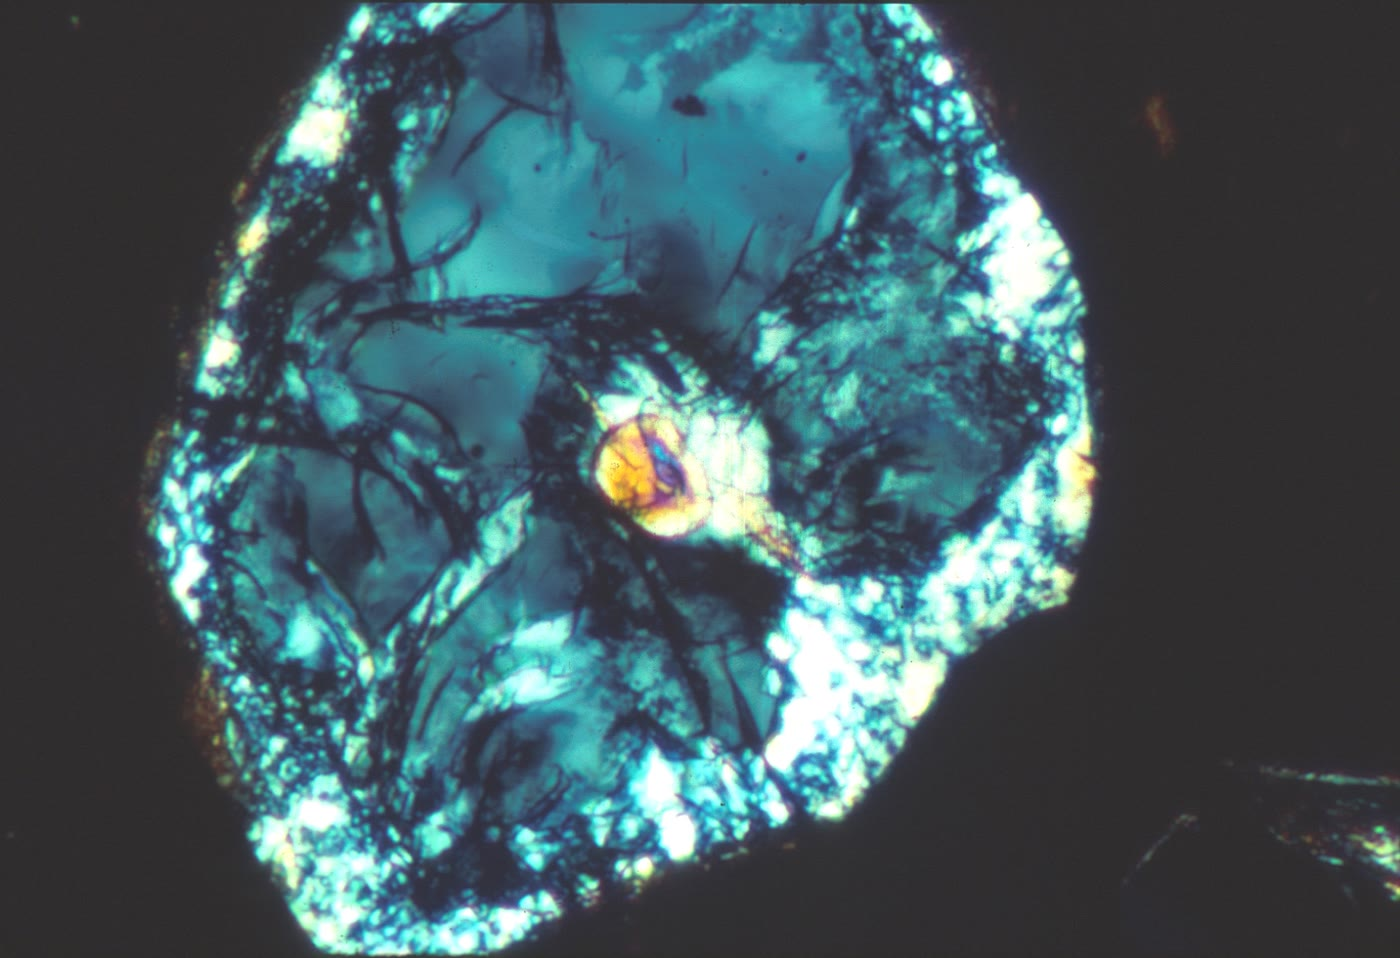
\includegraphics[width=0.62\linewidth]{images/book4/b2-11-coesite.jpg}
\par\smallskip{\small Coésite dans une éclogite, d'environ \qty{1}{mm} de diamètre, dans une lame mince
entre polariseurs croisés~: le grand grain central est de la coésite, la couronne de petits grains clairs est
du quartz né à partir d'elle lorsque la pression a baissé~; le petit grain coloré au centre est une
inclusion de pyroxène. Photographie J.\,R. Smyth, CC BY-SA 1.0.}
\end{omfigure}

Six ans plus tard, des diamants de \qty{12}{\micro m} en moyenne furent trouvés dans des gneiss, des schistes et
des roches à grenat et pyroxène du massif de Kokchetav, dans le nord du Kazakhstan, enfermés dans du grenat
et du zircon, qui les protégeaient de la transformation en graphite~: ils ont cristallisé à \qty{40}{kbar}
ou plus et au-dessus de 900 à \qty{1000}{\celsius}. La croûte continentale, pourtant légère, peut être
entraînée à plus d'une centaine de kilomètres de profondeur.
% ledger: ss90:diamond

Le retour se lit dans ses horloges. Dans les roches subduites les plus profondes des Alpes,
la titanite datée à des stades successifs montre qu'une roche calco-silicatée a atteint environ
\qty{3.5}{GPa} à $35.1 \pm \qty{0.9}{Ma}$, se trouvait à $1 \pm \qty{0.15}{GPa}$ à $32.9 \pm
\qty{0.9}{Ma}$, et vers 0.4 à \qty{0.5}{GPa} à $31.8 \pm \qty{0.5}{Ma}$. Les
vitesses moyennes d'\omterm{def:b2:pt-paths:exhumation}{exhumation}, 3.4 puis \qty{1.6}{cm.an^{-1}}, correspondent aux vitesses des plaques~: les roches
sont remontées à peu près aussi vite qu'elles étaient descendues, bien plus vite que l'érosion n'aurait pu les
découvrir. Les auteurs invoquent la flottabilité, la croûte légère remontant à travers le manteau plus dense, et
des failles normales, qui amincissent les roches au-dessus.
% ledger: rh01:exhumation

\section{Métamorphisme océanique}\label{sec:b2:pt-paths:ocean-floor}

\begin{definition}[Métamorphisme océanique~; serpentinisation]\label{def:b2:pt-paths:ocean-floor}
\emph{Métamorphisme océanique}\index{métamorphisme océanique} est le \omterm{def:b2:metamorphic-facies:metamorphism}{métamorphisme} régional de la
lithosphère océanique près des dorsales, par des fluides aqueux chauds
circulant sous de forts gradients géothermiques~; la recristallisation est en général incomplète
et la température augmente en général avec la profondeur. La \emph{serpentinisation}\index{serpentinisation}
est l'hydratation de roches riches en olivine en serpentine.
\end{definition}
% ledger: scmr:types

L'eau de mer aspirée dans la jeune croûte près de l'axe d'une dorsale se réchauffe, réagit avec les roches et
remonte. Les basaltes qu'elle traverse recristallisent, de façon incomplète, en minéraux hydratés
sur une large gamme de températures. Là où l'eau atteint la \omterm{def:b2:mantle-melting:peridotites}{péridotite}, comme sur
les dorsales lentes où la roche du manteau affleure au fond de la mer et alimente des sources comme
celles du champ de Lost City (volume de première année universitaire), l'olivine fixe de l'eau~:
\[
\ce{2 Mg2SiO4 + 3 H2O -> Mg3Si2O5(OH)4 + Mg(OH)2},
\]
la forstérite donnant serpentine et brucite. Les volumes molaires, 43.65 pour la forstérite, 107.50
pour la serpentine et \qty{24.63}{cm^3.mol^{-1}} pour la brucite, montrent ce que cela fait à la roche~:
\qty{87.30}{cm^3} d'olivine deviennent \qty{132.13}{cm^3} de solides, soit \qty{51}{\percent}
de plus, et la masse volumique tombe de 3.22 à \qty{2.54}{g.cm^{-3}}. La roche gonfle et
s'allège, et l'eau qu'elle a fixée descend avec elle lorsque la plaque est subduite.
% ledger: scmr:types, rh95:serpentine, kelley:lost-city, dick:ultraslow

\begin{inthelab}[Lire un grenat]
Pour lire un \omterm{def:b2:pt-paths:paths}{chemin P--T}, un pétrologue découpe d'abord une lame mince passant par le centre d'un
grenat, car une coupe excentrée manque le cœur. Au microscope, les inclusions
sont cartographiées~: de petits grains de quartz, de biotite, de plagioclase ou de disthène piégés pendant la croissance du grenat,
parfois alignés en traînées qui conservent une foliation plus ancienne de la roche. Une microsonde électronique
mesure ensuite la composition le long d'une ligne allant du cœur à la bordure, et une cartographie du
magnésium, du fer, du calcium et du manganèse montre les zones de croissance. Chaque zone est associée aux
minéraux qui ont cristallisé avec elle~: les inclusions pour le cœur, la matrice en contact pour la
bordure. Le thermomètre et le baromètre sont appliqués à chaque couple, et les zones sont datées
lorsqu'un minéral le permet. \Cref{ch:b2:field-lab-methods-2} décrit les instruments.
\end{inthelab}

\begin{omfigure}
\centering
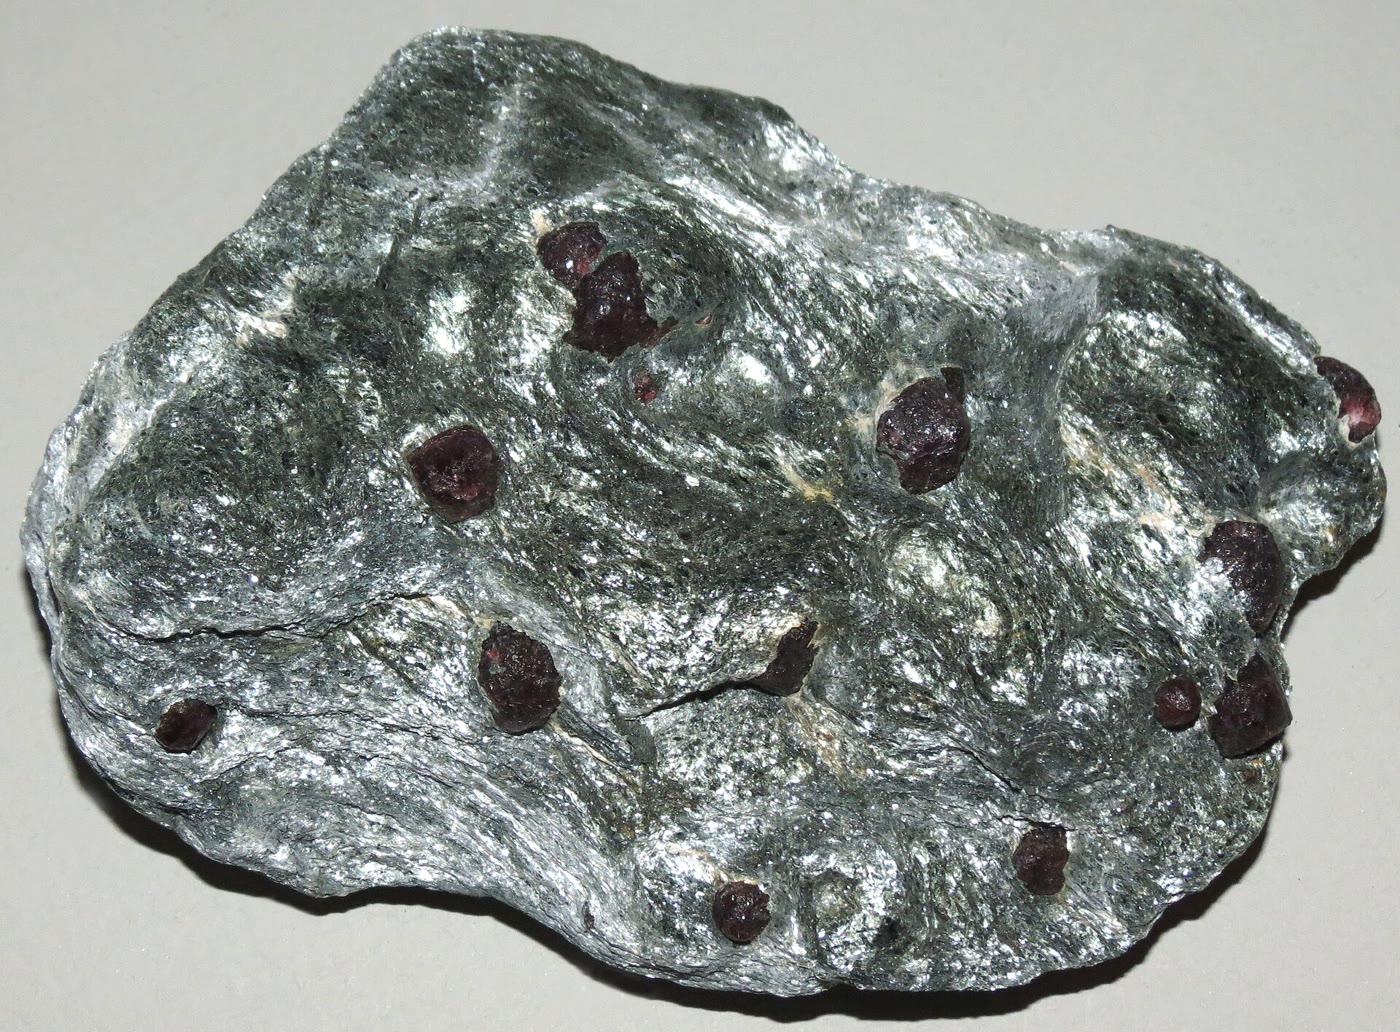
\includegraphics[width=0.62\linewidth]{images/book4/b2-11-garnet-schist.jpg}
\par\smallskip{\small Un schiste à grenat~: cristaux de grenat rouge sombre, formés dans une matrice foliée
de micas. Chaque grenat peut conserver, du cœur à la bordure, une
trace du chemin de la roche. Photographie James St.~John, CC BY 2.0.}
\end{omfigure}

\section{Exercices}

\begin{exercise}[$\star$]\label{exo:b2:pt-paths:1}
Six échantillons d'une même formation d'argilites, prélevés le long d'une route, contiennent~: (A) chlorite,
muscovite, quartz~; (B) biotite, chlorite, muscovite, quartz~; (C) grenat, biotite,
muscovite, quartz~; (D) staurolite, grenat, biotite, muscovite, quartz~; (E) disthène,
staurolite, biotite, muscovite, quartz~; (F) sillimanite, biotite, muscovite, quartz.
(a) Dans quelle zone de Barrow se situe chacun~? (b) Combien d'isogrades la route traverse-t-elle, et
lesquels~? (c) Pourquoi ne suffit-il pas de connaître les isogrades pour tracer le \omterm{def:b2:pt-paths:barrovian}{gradient
métamorphique de terrain}~?
\end{exercise}
% ledger: iugs:barrow

\begin{exercise}[$\star$]\label{exo:b2:pt-paths:2}
Un grenat a $X_{\text{Mg}} = 0.10$ et $X_{\text{Fe}} = 0.80$, la biotite qui le jouxte
a $X_{\text{Mg}} = 0.45$ et $X_{\text{Fe}} = 0.50$. (a) Calculer $K_D$ et $\ln K_D$.
(b) Avec la calibration de ce chapitre, calculer la température à \qty{5}{kbar} et à
\qty{7}{kbar}. (c) Le couple est-il un thermomètre ou un baromètre~?
\end{exercise}
% ledger: h97:ideal, h97:fs-reaction

\begin{exercise}[$\star$]\label{exo:b2:pt-paths:3}
Une \omterm{def:b2:metamorphic-facies:protoliths}{métapélite} donne \qty{580}{\celsius} et \qty{6.0}{kbar}. (a) Sous des roches de masse volumique
moyenne \qty{2800}{kg.m^{-3}} ($g = \qty{9.81}{m.s^{-2}}$), à quelle profondeur se trouvait-elle~? (b) Quel
gradient de température cela implique-t-il depuis \qty{10}{\celsius} en surface~? (c) La
droite expérimentale disthène $=$ sillimanite passe par \qty{3.67}{kbar} à
\qty{500}{\celsius} et \qty{5.77}{kbar} à \qty{600}{\celsius}~: quel aluminosilicate
la roche doit-elle contenir~?
\end{exercise}
% ledger: hm93:table11

\begin{exercise}[$\star$]\label{exo:b2:pt-paths:4}
Pour la \omterm{def:b2:pt-paths:ocean-floor}{serpentinisation} de la forstérite écrite dans ce chapitre~: (a) vérifier que l'équation
est équilibrée en masse, avec des masses molaires de 140.693 (forstérite), 18.015 (eau),
277.112 (serpentine) et \qty{58.320}{g.mol^{-1}} (brucite)~; (b) calculer la variation de
volume des solides~; (c) calculer les masses volumiques de l'olivine et des produits.
(d) Que fait cette variation à une \omterm{def:b2:mantle-melting:peridotites}{péridotite} serpentinisée sous le fond de la mer~?
\end{exercise}
% ledger: rh95:serpentine

\begin{exercise}[$\star\star$]\label{exo:b2:pt-paths:5}
Calibrer le thermomètre à partir de quatre expériences à \qty{2.07}{kbar}~: $\ln K_D =
-1.157$ et $-1.255$ à \qty{799}{\celsius}, $-1.738$ et $-1.826$ à \qty{550}{\celsius}.
(a) Calculer la moyenne de chaque couple et trouver la droite $\ln K_D = a/T + b$ passant par les deux moyennes.
(b) En déduire $\Delta_r H$ et $\Delta_r S$, avec $\Delta_r V = \qty{0.311}{J.bar^{-1}}$.
(c) Comparer les températures que donnent votre calibration et celle du chapitre à
\qty{5}{kbar} pour $K_D = 0.18$, $0.10$ et $0.30$. Que concluez-vous sur
l'extrapolation d'une calibration~?
\end{exercise}
% ledger: h97:fs-data, h97:ideal

\begin{exercise}[$\star\star$]\label{exo:b2:pt-paths:6}
(a) À partir des volumes molaires à \qty{298}{K} (almandin 115.32, pyrope 113.12, annite
154.30, phlogopite 149.65, grossulaire 125.28, anorthite 100.79, disthène 44.15, quartz
\qty{22.69}{cm^3.mol^{-1}}), calculer $\Delta_r V$ de l'échange et de la réaction GASP,
et comparer aux valeurs qu'utilisent les calibrations, \num{0.311} et
\qty{-6.21}{J.bar^{-1}}. (b) Pour $K_D = 0.18$, de combien de kelvins une erreur de
\qty{1}{kbar} décale-t-elle la température~? (c) Le long de la droite GASP d'une roche dont
$X_{\text{Ca}}/X_{\text{an}} = 0.20$, de combien de bars une erreur de \qty{17}{K} décale
la pression~?
\end{exercise}
% ledger: rh95:gb-gasp, rh95:al2sio5, h97:fs-reaction, kn88:gasp

\begin{exercise}[$\star\star$]\label{exo:b2:pt-paths:7}
À \qty{600}{\celsius}, un grenat a $X_{\text{Ca}} = 0.08$ et le plagioclase qui le jouxte
$X_{\text{an}} = 0.30$. (a) Calculer la pression GASP. (b) Refaire le calcul avec $X_{\text{an}} =
0.35$. (c) À quelle profondeur se trouvait la roche, pour une masse volumique moyenne de \qty{2800}{kg.m^{-3}}~?
\end{exercise}
% ledger: kn88:gasp

\begin{exercise}[$\star\star$]\label{exo:b2:pt-paths:8}
Utiliser les âges à la titanite des roches subduites les plus profondes des Alpes~: environ \qty{3.5}{GPa} à
$35.1 \pm \qty{0.9}{Ma}$, \qty{1.0}{GPa} à $32.9 \pm \qty{0.9}{Ma}$, \qty{0.45}{GPa} à
$31.8 \pm \qty{0.5}{Ma}$. (a) Avec une masse volumique moyenne de \qty{3000}{kg.m^{-3}}, convertir les
pressions en profondeurs. (b) Calculer les deux vitesses moyennes d'\omterm{def:b2:pt-paths:exhumation}{exhumation} et les comparer aux
valeurs publiées, 3.4 et \qty{1.6}{cm.an^{-1}}. (c) Quelle est l'incertitude du premier intervalle de temps,
et quelle gamme de vitesses permet-elle~? (d) Comparer à la vitesse d'érosion du
modèle d'épaississement, \qty{0.5}{mm.an^{-1}}.
\end{exercise}
% ledger: rh01:exhumation

\begin{exercise}[$\star\star$]\label{exo:b2:pt-paths:9}
Pour $K_D = 0.18$ à \qty{5}{kbar}, (a) calculer $\partial T/\partial\ln K_D$ et
$\partial T/\partial P$ à partir de la proposition~; (b) avec $\sigma_{\ln K_D} = 0.05$ (une
erreur de \qty{5}{\percent} sur $K_D$) et $\sigma_P = \qty{1}{kbar}$, calculer $\sigma_T$.
(c) Quelle erreur domine~? Comparer à l'incertitude de \qty{25}{\celsius} revendiquée pour
les meilleures calibrations.
\end{exercise}
% ledger: h97:ideal

\begin{exercise}[$\star\star\star$]\label{exo:b2:pt-paths:10}
Une bordure de grenat a $X_{\text{Mg}} = 0.10$, $X_{\text{Fe}} = 0.75$, $X_{\text{Ca}} = 0.07$~;
la biotite de la matrice $X_{\text{Mg}} = 0.42$, $X_{\text{Fe}} = 0.52$~; le plagioclase
$X_{\text{an}} = 0.25$. (a) Appliquer la méthode de ce chapitre, en partant de \qty{6}{kbar},
jusqu'à ce que la température change de moins de \qty{1}{K}. (b) Quel aluminosilicate doit
la roche contenir (utiliser la droite expérimentale de l'\cref{exo:b2:pt-paths:3})~? (c) Pourquoi le baromètre doit-il utiliser
l'aluminosilicate réellement présent~?
\end{exercise}
% ledger: h97:ideal, kn88:gasp, hm93:table11

\begin{exercise}[$\star\star\star$]\label{exo:b2:pt-paths:11}
Avec $\kappa = \qty{1e-6}{m^2.s^{-1}}$~: (a) calculer le temps de relaxation de la
proposition pour $L = \qty{35}{km}$ et pour $L = \qty{70}{km}$. (b) Le modèle érode
\qty{35}{km} en 70 millions d'années~; comparer ce temps à ceux de (a). (c) Expliquer,
à partir de ces temps, pourquoi la roche du modèle atteint son pic thermique après son pic de
pression. (d) Si l'érosion était dix fois plus rapide, que changerait-il dans le chemin~?
\end{exercise}
% ledger: delaney:conductivity, et84:ptt

\begin{exercise}[$\star\star\star$]\label{exo:b2:pt-paths:12}
Prenons une croûte de \qty{35}{km} d'épaisseur et de masse volumique \qty{2800}{kg.m^{-3}}, au-dessus d'un manteau de
\qty{3300}{kg.m^{-3}}. (a) À quelle profondeur la pression atteint-elle \qty{28}{kbar}, le
minimum pour la coésite de Dora Maira~? (b) Et \qty{40}{kbar}, pour les diamants de Kokchetav~?
(c) Quel gradient moyen implique \qty{700}{\celsius} à la profondeur de (a), et dans quelle
série se range-t-il~? (d) À \qty{3.4}{cm.an^{-1}}, combien de temps dure la remontée depuis la profondeur
de (a) jusqu'à \qty{35}{km}~?
\end{exercise}
% ledger: chopin84:coesite, ss90:diamond, rh01:exhumation

\section{Problème~: le voyage d'un grenat}

\begin{problem}[{Problème de fin de semaine --- thermobarométrie, chemin et vitesse d'exhumation d'un
schiste}]
\label{pb:b2:pt-paths:1}
Un schiste à disthène--grenat--biotite renferme des grenats avec un cœur et une bordure. Le cœur enferme
de la biotite, du plagioclase et de la disthène~; la bordure touche la biotite et le plagioclase de la
matrice. Autour des grenats, une partie de la disthène est remplacée par de la sillimanite, et aux bords des grenats
a poussé de la chlorite. Les analyses sont~:
\begin{center}
\small
\begin{tabular}{@{}lccc@{}}
\hline
& $X_{\text{Mg}}$ & $X_{\text{Fe}}$ & $X_{\text{Ca}}$ ou $X_{\text{an}}$\\
\hline
cœur de grenat & 0.080 & 0.760 & 0.050\\
biotite incluse dans le cœur & 0.40 & 0.58 & ---\\
plagioclase inclus dans le cœur & --- & --- & 0.25\\
bordure de grenat & 0.120 & 0.720 & 0.060\\
biotite de la matrice & 0.46 & 0.53 & ---\\
plagioclase de la matrice & --- & --- & 0.28\\
\hline
\end{tabular}
\end{center}
Utiliser le thermomètre grenat--biotite et le baromètre GASP de ce chapitre (mélange idéal),
$R = \qty{8.314}{J.mol^{-1}.K^{-1}}$, $g = \qty{9.81}{m.s^{-2}}$, une masse volumique moyenne de
\qty{2800}{kg.m^{-3}} au-dessus de la roche, et arrondir chaque rapport à quatre décimales.

\noindent\textbf{Partie I --- Températures.}
\begin{enumerate}
\item Calculer $X_{\text{Mg}}/X_{\text{Fe}}$ dans le cœur du grenat et dans la biotite incluse,
puis $K_D$ et $\ln K_D$ pour le cœur.
\item Faire de même pour la bordure et la biotite de la matrice.
\item Calculer la température du cœur à \qty{6}{kbar}.
\item Calculer la température de la bordure à \qty{6}{kbar}.
\item De combien de kelvins une erreur de \qty{1}{kbar} changerait-elle ces températures~?
\item Pourquoi le cœur est-il associé à la biotite incluse, et la bordure à la biotite de la
matrice~?
\end{enumerate}

\noindent\textbf{Partie II --- Pressions.}
\begin{enumerate}[resume]
\item Calculer la pression du pôle $P_0$ de la réaction GASP aux deux températures
des questions~3 et~4.
\item Calculer la pression GASP du cœur à la température de la question~3.
\item Calculer la pression GASP de la bordure à la température de la question~4.
\item Recalculer la température de la bordure à la pression de la question~9, puis sa
pression à cette température, et une nouvelle fois la température. Donner la température et la
pression de la bordure.
\item Faire de même une fois pour le cœur. Pourquoi change-t-il si peu~?
\item Convertir les pressions du cœur et de la bordure en profondeurs.
\item La droite expérimentale disthène $=$ sillimanite passe par 3.67, 5.77 et
\qty{7.86}{kbar} à 500, 600 et \qty{700}{\celsius}. Quel aluminosilicate était stable
quand le cœur a cristallisé, et quand la bordure a cristallisé~? La disthène du cœur est-elle cohérente~?
\end{enumerate}

\noindent\textbf{Partie III --- Le chemin.}
\begin{enumerate}[resume]
\item Entre le cœur et la bordure, de combien la température et la pression ont-elles changé~?
Le grenat croissait-il sur le \omterm{def:b2:pt-paths:paths}{chemin prograde} ou sur le \omterm{def:b2:pt-paths:paths}{chemin rétrograde}~?
\item La sillimanite remplace la disthène autour des grenats. À la température de la bordure,
en dessous de quelle pression la roche a-t-elle dû passer pour que cela se produise~? Que fit la roche
après la croissance de la bordure~?
\item La chlorite croît aux bords des grenats. Quelle partie du chemin enregistre-t-elle~?
\item Tracer le chemin~: cœur, bordure, sillimanite, chlorite. Est-il horaire ou antihoraire~?
Quel pic est survenu en premier~?
\item Le modèle d'épaississement de ce chapitre amène sa roche à un pic thermique de
\qty{593}{\celsius} à \qty{7.8}{kbar}. Le chemin du schiste est-il de même nature~?
\end{enumerate}

\noindent\textbf{Partie IV --- À quelle vitesse.}
\begin{enumerate}[resume]
\item La bordure de grenat donne un âge samarium--néodyme de $412.0 \pm \qty{1.5}{Ma}$, pris
comme âge du pic~; une muscovite de la matrice donne un âge argon de $398.0 \pm
\qty{1.0}{Ma}$, moment où la roche a refroidi à travers \qty{405}{\celsius}. Calculer
la vitesse moyenne de refroidissement entre les deux.
\item La température de fermeture de \qty{405}{\celsius} suppose un refroidissement à
\qty{10}{\celsius} par million d'années. La vitesse de la question~19 appelle-t-elle une valeur plus élevée ou plus
basse, et pourquoi~?
\item À \qty{398}{Ma}, prendre un géotherme de \qty{30}{\celsius\per\km} depuis
\qty{10}{\celsius} en surface. À quelle profondeur la muscovite s'est-elle fermée~?
\item De combien la roche est-elle remontée entre le pic et la fermeture de la muscovite~?
\item Quelle est l'incertitude de l'intervalle de temps~?
\item Calculer la vitesse moyenne d'\omterm{def:b2:pt-paths:exhumation}{exhumation} du pic à la fermeture de la muscovite, en
millimètres par an et arrondie au dixième~: le nombre clé de ce problème.
\end{enumerate}
\end{problem}
% ledger: h97:ideal, h97:fs-reaction, kn88:gasp, hm93:table11, h09:muscovite, scmr:ptt, et84:ptt
